\chapter{Sensors and measurements}

\textbf{Author: Lukas Leskovar} 

The means of perceiving ones surrounding environment are a crucial part of any robotic system. This chapter aims to describe the need for interoceptive measurements aiding the different algorithms used within Autumn as well as any sensory equipment supporting such data acquisition. To this end the underlying principles and concepts behind the measurement techniques and  are illustrated.

\section{Motion Models}
Kinematic models in robotics are used for describing and planning state-transitions between consecutive robot poses. While Chapter \ref{chapter:slam} focuses on the theoretic basics of such models and how to build upon them, this section is going to focus on the practical concepts used in robot localization. To this end classical odometry as well as velocity based motion models are described.
To facilitate any equations later in this section the robot pose is described by its state vector 
\[
\begin{pmatrix}
	x \\
	y \\
	\theta \\
\end{pmatrix}
\] 
which defines its position as Cartesian coordinates and bearing as angular orientation $\theta$ in 2 dimensional space. 

\subsection{Odometry}
Ben-Ari and Mondada define this topic as follows: "Odometry—the measurement of distance—is a fundamental method used by robots for navigation.". \footcite[Page 69]{ben2017elements} 
When performing linear odometry, e.g. without taking orientation changes into consideration, this distance is calculated rather trivially by inferring it through measured time elapsed and the velocity of the robot proportionally to the motor power. 
Other systems however utilize wheel encoders to count the number of wheel rotations thus allowing for rather precise estimation of distance. 

With non-linear motion the distances $d_{l}$ and $d_{r}$ moved by the left and right wheel are unequal which requires the calculation of both updated position and bearing of the robot. 
Lets suppose a robot moved from position $\begin{pmatrix} x & y & \theta \end{pmatrix}^{T}$ to $\begin{pmatrix} x' & y' & \theta' \end{pmatrix}^{T}$ with a slight left turn caused by the right wheel turning faster than the left one. 
This scenario is depicted in Fig. \ref{fig:odom} with $\varphi$ corresponding to the turn angle in radians, the radii $r_{l}, r_{c}, r_{r}$ describing the distance from the new position of the wheels and center to point $P$, the origin of the turn. 

For small angles these radii are approximately the same length as the distances $d_{l}, d_{c}$ and $d_{r}$, which allows for the turn angle to be calculated as follows:
\begin{align*}
	\varphi &= \frac{d_{i}}{r_{i}}, & i &= l, r, c  
\end{align*}

However in practical scenarios where these radii and the point P are unknown, $\varphi$ has to be calculated only using $d_{l}$, $d_{r}$ and $b$ which corresponds to the distance between both robot wheels.

\begin{equation*}
	\begin{split}
		\varphi r_{r} = d_{r} \\
		\varphi r_{l} = d_{l} \\
		\varphi r_{r} - \varphi r_{l} = d_{r} - d_{l} \\
		\varphi = \frac{d_{r} - d_{l}}{r_{r} - r_{l}} \\ 
		\varphi = \frac{d_{r} - d_{l}}{b} \\
	\end{split}
\end{equation*}

To calculate the new coordinate positions the distance $d_{c}$ is computed:
\begin{equation*}
	d_{c} = \frac{d_{l} + d_{r}}{2}
\end{equation*}

The final pose is calculated as follows:

\begin{equation*}
	\begin{pmatrix}
		x' \\ 
		y' \\
		\theta'
	\end{pmatrix}
	= 
	\begin{pmatrix}
		-d_{c} \sin \varphi \\
		d_{c} \cos \varphi \\ 
		\theta + \varphi
	\end{pmatrix}
\end{equation*}

Because the assumptions above only apply for small distances in any real-world systems such computations ought to be performed continuously. However due to uncertain measurements these calculations inherit some margin of error which is integrated up over multiple iterations thus causing a slight drift in the output.\footcite[Pages 69 - 77]{ben2017elements} 
This drift can be corrected using techniques discussed in Chapter \ref{chapter:slam}.

\begin{figure}
	\centering
	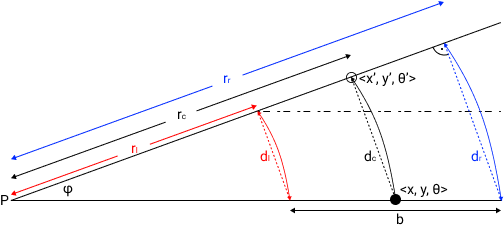
\includegraphics[width=0.8\linewidth]{img/odom}
	\caption{
		This diagram shows the geometry of how a slight turning motion can be calculated only using the distances $d_{l}$, $d_{r}$ and wheel offset $b$.
		The robot pose 
		$
			\begin{pmatrix}
				x &
				y &
				\theta 
			\end{pmatrix}^{T}
		$
		is associated with the center of the robot \footcite{ben2017elements}.
	}
	\label{fig:odom}
\end{figure}


\subsection{Inertial Measurement}
Another way of modelling motion usually utilized when a robot is not equipped with wheel encoder nor wheels is based on velocities influencing the vehicle. Typically the inputs of velocity based motion models are measured used Inertial Measurement Units (IMU), Gyroscopes and Accelerometers. 

These velocities $v$ and $\omega$ denote the linear and angular velocity and are referred to as controls for the system. 
In contrast to odometry which can only be calculated after a movement has been performed these controls allow for prior motion planning. \footcite[Pages 92 - 99]{thrun2002probabilisticRobotics}

If these velocities stay fixed for the entire duration $\Delta t$ of the motion from 
$\begin{pmatrix} x & y & \theta \end{pmatrix}^{T}$
to
$\begin{pmatrix} x' & y' & \theta' \end{pmatrix}^{T}$
the robot moves in a circle with radius $r$ as seen in Fig. \ref{fig:inertial}. The center $P$ of this circle with coordinates 
$
\begin{pmatrix}
	x_{P} & y_{P}
\end{pmatrix}
^{T}
$
can be evaluated as follows:

\begin{equation}
	\begin{split}
		x_{P} = x - \frac{v}{\omega} \sin \theta \\
		y_{P} = y + \frac{v}{\omega} \cos \theta
	\end{split}
\end{equation}

This allows for the new position to be calculated: 

\begin{equation}
	\begin{pmatrix}
		x' \\
		y' \\
		\theta'
	\end{pmatrix}
	=
	\begin{pmatrix}
		x_{P} + \frac{v}{\omega} \sin(\theta + \omega \Delta t) \\
		y_{P} - \frac{v}{\omega} \cos(\theta + \omega \Delta t) \\
		\theta + \omega \Delta t
	\end{pmatrix}
\end{equation}

Despite incapable of calculating movements in advance, odometry ought to be preferred over velocity motion models as they pose higher accuracy in localization. \footcite[Page 107]{thrun2002probabilisticRobotics}

\begin{figure}
	\centering
	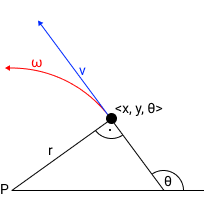
\includegraphics[width=0.5\linewidth]{img/inertial}
	\caption{
		In this diagram a slight turning motion of the robot is described by the translational velocity $v$ and angular velocity $\omega$. These velocities, if remaining unchanged, render the robot to move in a perfect circle with the center point $P$ and radius $r = | \frac{v}{\omega}|$. Even if the angular velocity remains 0 the motion is still described as a circle with an infinite radius. \footcite[Pages 95 - 107]{thrun2002probabilisticRobotics}
	}
	\label{fig:inertial}
\end{figure}



\section{Depth Sensing}
Similar to motion models contributing to robot localization in Autumn, Depth Sensing is utilized to perceive and map the drones environment. 
The technologies in this section focus on mapping distance information to each point in the cameras field of view thus providing 3D-Imaging.

\subsection{Structured Light}
One approach uses active illumination to project a varying intensity pattern onto the perceived scene thus allowing for a camera to extract 3D-information from the distorted pattern as the surface of the scene is non-planar. \footcite{geng2011StructuredLight}

\subsection{Time-of-Flight}
Time-of-Flight (ToF) sensors perform active triangulation, which is performed by emitting modulated light to be reflected by a scene, as described in Fig. \ref{fig:activeTriangulation}. The distance to the scene is determined using the time difference between emission and detection of singular rays (more prominent with ToF Laser-Scanners like LiDAR) or the phase shift of light reflected by the whole scene. The latter allows for mapping depth information to the entire Field-of-View (FoV) of a camera. 
%It may be necessary to differentiate mapping using depth perception sensors from LiDAR technologies which pose an alternative solution. 
Although LiDAR sensors fall under the category of ToF sensors they perceive the distance to an object using pulsed lasers thus outputting
the distance to singular points in the sensors environment rather than depth information mapped to an image. \footcite{gokturk2004time} \footcite{velodyne2021LiDAR}
% LiDAR verwenden die Zeitdifferenz und berechnen mittels Trigonometrie die Distanz
As 3D-LiDAR sensors applied in many commercial mapping solution are very expensive they disqualify for use in Autumn as it focuses on performing with approximate precision using relatively inexpensive camera based equipment. 

\begin{figure}
	\centering
	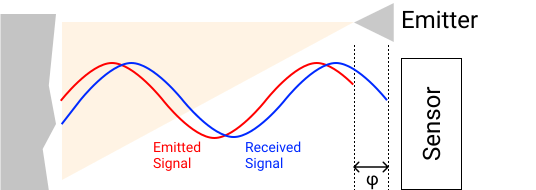
\includegraphics[width=0.8\linewidth]{img/activeTriangulation}
	\caption{
		This diagram depicts a ToF depth camera emitting IR-light (red) onto a surface. The camera sensor then utilizes the phase-shift $\varphi$ between the emitted (red) and received signal (blue) to calculate the distance between the scene and sensor. \footcite{altuntas2021triangulation}
		% noch mehr schreiben
	}
	\label{fig:activeTriangulation}
\end{figure}


\subsection{Stereo Vision}
The last and most significant approach to Autumn performs passive triangulation using two cameras setup as seen in Fig. \ref{fig:passiveTriangulation}. Although this eliminates the need for any light to be emitted, however the problem of correspondence is introduced, which deals with associating the different projections to the same point in the real world\footcite{ng2019StereoCorrespondence}. There are multiple approaches to this problem which are generally divided into global and local matching methods with the latter being more computationally efficient while sacrificing quality. \footcite{do2019review}

In Autumn this approach was pursued using a Stereolabs ZED depth camera as it was superior to any competitors such as the Microsoft Kinect or Intel Realsense concerning availability and cost-effectiveness. 

\begin{figure}
	\centering
	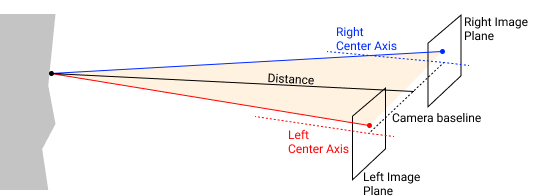
\includegraphics[width=0.8\linewidth]{img/PassiveTriangulation}
	\caption{
		This diagram describes the camera setup found in passive triangulation systems. Using stereo-photogrammetry the distance to the perceived scene is calculated.\footcite{altuntas2021triangulation}
	}
	\label{fig:passiveTriangulation}
\end{figure}

\subsection{ZED 1 vs ZED 2}
%As mentioned in Chapter \ref{chapter:architecture} the Stereolabs ZED 1 was used in a first prototype and later replaced with a 
Chapter \ref{chapter:architecture} mentions that the Stereolabs ZED 1 used in early prototypes was quickly replaced with the ZED 2. This change was due to processing limitations and additional features provided by the newer product version.
This section aims to benchmark the two cameras from a depth-performance standpoint to review if the upgrade enhanced depth perception thus improving the system output or if no changes were necessary when only considering depth-perception.

\subsubsection{Experiment}
To answer this question the cameras measured the vertical distance enclosed by two points mounted 1 m above each other on a stationary structure with the bottom one at a height 1 m above the ground. 
The cameras was paced on a movable rig normal to the stationary structure and 1m above the ground.  The aforementioned gap was measured by the cameras at 1 m increments between 3 m and 10 m horizontal distance measured amongst each structures base. 

The usage of ARUCO markers allowed for precisely tracking the position of each point within the camera coordinate system thus ensuring the points remain fixed even though the camera rig is moved. 
% über ARUCO schreiben
% reference zu ARUCO 
ARUCO markers are squared-based markers popular in many robotic and augmented reality applications as they provide a fast and robust solution for estimating a cameras pose. Each marker has a unique, identifiable pattern which allows for precisely determining and tracking its position.\footcite{jurado2015} 

\subsubsection{Results}
%Fig. \ref{plot:zedBenchmark} depicts the mean depth-perception error measured thus indicating how well each camera performed. 

The mean depth-perception error dependant on the camera distance for the ZED 1 (blue) is plotted in Fig. \ref{plot:zedBenchmark}. To illustrate the positive tendency a linear regression (cyan) is superimposed. The trend line indicates a relatively steep slope with the mean error adding up by 0.03 m at increasing distances from the rig. Additionally the error range listed in Tab. \ref{tab:errorMinimaMaxima} shows a base error of 0.7\% and a maximum mean error of 3\%, which is similar to the error stated by the cameras data sheet\footcite{zed1Datasheet}.

The data for the ZED 2 (red) and its corresponding trend line (orange) indicate a much more shallow slope with 0.01 m per meter distance to the rig. Looking at the error range the ZED 2 lies below 1\% mean error at all distances which also corresponds to the data sheets specifications \footcite{zed2Datasheet}.


%When comparing each trend line for each camera it is apparent that the slope of the ZED 1 with $0.03m/m$ is more than twice as large compared to the ZED 2 at $0.01m/m$. This indicates that with increasing distance the depth-perception error increases dramatically. 
%Another interesting finding are the minima and maxima of the mean depth-perception error found in Tab. \ref{tab:errorMinimaMaxima}.
%As illustrated the ZED 1 inherits a substantially large minimal and maximal error of  $0.07m$ and $0.31m$.
%Compared to this the ZED 2 performed much better with a almost non existent base error and a maximal error of $0.1m$.

\begin{table}[h]
	\centering
	\begin{tabular}{|l|l|l|}
		\hline
		& \textbf{Minimal Mean Error} & \textbf{Maximal Mean Error} \\ \hline
		\textbf{ZED 1}  & 0.07 m 					  & 0.31 m                      \\ \hline
		\textbf{ZED 2} & 0.01 m                      & 0.10 m                      \\ \hline
	\end{tabular}
	\caption{Table containing the minimal and maximal mean error of both the ZED 1 and ZED 2.}
	\label{tab:errorMinimaMaxima}
\end{table}

\begin{figure}[h]
	\begin{center}
		\begin{tikzpicture}
			\begin{axis}[
				width=0.8\linewidth, % Scale the plot to \linewidth
				grid=major, 
				grid style={dashed,gray!30},
				xlabel={Distance [m]}, % Set the labels
				ylabel={Mean Error [m]},
				legend pos=north west,
				xtick={3, 4, 5, 6, 7, 8, 9, 10},
				xmin=2,
				xmax=11,
				ymin=0,
				ymax=0.35,
				]
				
				
				%zed1 data
				\addplot[only marks, color=blue]
				table[row sep=crcr]{
					distance error \\
					0 0 \\
					3 0.072842 \\
					4 0.084444 \\
					5 0.090908 \\
					6 0.082350515 \\
					7 0.091252505 \\
					8 0.136357778 \\
					9 0.170380567 \\
					10 0.306662651 \\
				}; 
				\addlegendentry{ZED1}
				
				%zed1 regression
				\addplot[no marks, color=cyan, style=dashed]
				table[row sep=crcr, y={create col/linear regression={y=error}}]{
					distance error \\
					0 0 \\
					3 0.072842 \\
					4 0.084444 \\
					5 0.090908 \\
					6 0.082350515 \\
					7 0.091252505 \\
					8 0.136357778 \\
					9 0.170380567 \\
					10 0.306662651 \\
				};
				\addlegendentry{$y = 0.03x + 0.04; R^2 =  0.67$} 
				
				%zed2 data
				\addplot[only marks, color=red]
				table[row sep=crcr]{
					distance error \\
					0 0 \\
					3 0.005048 \\
					4 0.010964 \\
					5 0.058536585 \\
					6 0.080308 \\
					7 0.045865731 \\
					8 0.040048 \\
					9 0.102566462 \\
					10 0.081332636 \\
				}; 
				\addlegendentry{ZED2}
				
				%zed2 regression
				\addplot[no marks, color=orange, style=dashed]
				table[row sep=crcr, y={create col/linear regression={y=error}}]{
					distance error \\
					0 0 \\
					3 0.005048 \\
					4 0.010964 \\
					5 0.058536585 \\
					6 0.080308 \\
					7 0.045865731 \\
					8 0.040048 \\
					9 0.102566462 \\
					10 0.081332636 \\
				}; 
				\addlegendentry{$y = 0.01x + 0.02; R^2 =  0.58$}
			\end{axis}
		\end{tikzpicture}
		\caption{This plot describes how the mean depth-performance error of both the ZED 1 (blue) and ZED 2 (red) Stereo Camera changes with increasing distance to an object. Furthermore the linear regression function for both the ZED 1 (cyan) and ZED 2 (orange) are plotted. 
		 }
	 	\label{plot:zedBenchmark}
	\end{center}
\end{figure}


Comparing both trend lines and mean error range the ZED 1 clearly shows a much more aggressive upwards trend and higher base error compared to the ZED 2. However as the coefficient of determination $R^{2}$ for each trend line indicate a mediocre fit the aforementioned assumptions should not be solely taken into consideration when comparing the two camera systems. 
Having said this, in combination with the data sheets, the overall trend on depth-performance meets the initial assumption and justifies the upgrade to the ZED 2.

%Considering all of the aforementioned findings it is apparent that the ZED 2 produced much better depth-perception results compared to the ZED 1. This justifies the upgrade not only from a feature focused standpoint but also quality wise as this greatly effects the final 3D point cloud utilized by components discussed later in this thesis. 

\filbreak